\documentclass[11pt,letterpaper]{article}

\usepackage[margin=1in,headheight=14pt]{geometry}
\usepackage{amsmath,amssymb,amsthm,mathtools}
\usepackage{graphicx}
\usepackage{xcolor}
\usepackage{enumitem}
\usepackage{microtype}
\usepackage{fancyhdr}
\usepackage{bm}
\usepackage[colorlinks=true,linkcolor=blue,citecolor=blue,urlcolor=blue]{hyperref}

% Personal notation and theorem environments.
%!TEX root = EM_singular_models.tex

% PDF margin etc settings
%\setlength{\textwidth}{\paperwidth}
%\addtolength{\textwidth}{-6cm}
%\setlength{\textheight}{\paperheight}
%\addtolength{\textheight}{-4cm}
%\addtolength{\textheight}{-1.1\headheight}
%\addtolength{\textheight}{-\headsep}
%\addtolength{\textheight}{-\footskip}
%\setlength{\oddsidemargin}{0.5cm}
%\setlength{\evensidemargin}{0.5cm}

%%%%%%%%%%%%%%%%%%%%%%%%%%%%%%%%

% MACROS HERE

%%%%%%%%%%%%%%%%%%%%%%%%%%%%%%%%

\newcommand{\fixedpointtheta}{\widehat\theta_\obs}

\newcommand{\cover}{N}
\newcommand{\kinit}{\nu}
\newcommand{\cdelta}{c_\threshold}
\newcommand{\dndelta}{\omega}
\newcommand{\kndelta}{\Upsilon}
\newcommand{\kndeltanew}{\Psi}
\newcommand{\radii}{\mathcal{R}}
\newcommand{\event}{\mathcal{E}}
\newcommand{\kevent}{\mathcal{D}}


% Observations, dimension etc.
\newcommand{\dims}{\ensuremath{d}}
\newcommand{\samples}{\ensuremath{n}}
\newcommand{\obs}{\samples}
\newcommand{\real}{\ensuremath{\mathbb{R}}}
\newcommand{\complex}{\ensuremath{\mathbb{C}}}
\newcommand{\realdim}{\ensuremath{\real^\dims}}

\newcommand{\smallthreshold}{\epsilon}

% some mathcal notations
\newcommand{\order}[1]{\ensuremath{\mathcal{O}\parenth{#1}}}

% Basic statistics notation
\newcommand{\xstar}{\ensuremath{x^*}}
\newcommand{\xbar}{\ensuremath{\bar{x}}}
% True parameter
\newcommand{\thetastar}{\ensuremath{{\theta^*}}}
% Estimate one
\newcommand{\thetahat}{\ensuremath{\widehat{\theta}}}
% Estimate two
\newcommand{\thetatil}{\ensuremath{\widetilde{\theta}}}
\newcommand{\thetabar}{\ensuremath{\bar{\theta}}}
\newcommand{\yvec}{\ensuremath{y}}
\newcommand{\Xmat}{\ensuremath{X}}

% Distributions
\newcommand{\distribution}{P}
\newcommand{\density}{f}
\newcommand{\gaussiandensity}{\phi}
\newcommand{\NORMAL}{\ensuremath{\mathcal{N}}}
\newcommand{\BER}{\ensuremath{\mbox{Ber}}}

% Spaces
\newcommand{\Xspace}{\ensuremath{\mathcal{X}}}
\newcommand{\Yspace}{\ensuremath{\mathcal{Y}}}
\newcommand{\Zspace}{\ensuremath{\mathcal{Z}}}


% Brackets Size
\newcommand{\brackets}[1]{\left[ #1 \right]}
\newcommand{\parenth}[1]{\left( #1 \right)}
\newcommand{\bigparenth}[1]{\big( #1 \big)}
\newcommand{\biggparenth}[1]{\bigg( #1 \bigg)}
\newcommand{\braces}[1]{\left\{ #1 \right \}}
\newcommand{\abss}[1]{\left| #1 \right |}
\newcommand{\angles}[1]{\left\langle #1 \right \rangle}
\newcommand{\tp}{^\top}

% Generic vectors and scalars
\newcommand{\myvec}{u} % for generic vector
\newcommand{\myvectwo}{v} % for generic vector
\newcommand{\mymat}{B}
\newcommand{\set}{{A}}
\newcommand{\scalar}{\alpha}
\newcommand{\tvscalar}{\epsilon}
\newcommand{\tailboundscalar}{t}
\newcommand{\term}{U}
\newcommand{\myVarone}{\alpha_X}
\newcommand{\myVartwo}{\alpha_Y}
\newcommand{\myCovmat}{\Sigma}
\newcommand{\xcord}[1]{x^{(#1)}}
\newcommand{\xcordpop}[1]{X^{(#1)}}
\newcommand{\ycordpop}[1]{Y^{(#1)}}
\newcommand{\myVarthree}{\ensuremath{U}}
\newcommand{\myVarfour}{\ensuremath{V}}
\newcommand{\myfuntwo}{\ensuremath{g}}
\newcommand{\numsteps}{t}
\newcommand{\totalnumsteps}{T}
\newcommand{\seqalpha}[1]{\alpha_{#1}}
\newcommand{\seqnu}[1]{\nu^{(#1)}}
\newcommand{\imax}{\ell_\smallthreshold}
\newcommand{\basis}{e}
\newcommand{\radem}{\varepsilon}
\newcommand{\Tone}{T\ensuremath{_{0}}}
\newcommand{\Ttwo}{T\ensuremath{_{2}}}
\newcommand{\contractPar}[1]{\ensuremath{\gamma\parenth{#1}}}

\newcommand{\simiid}{\overset{\mathrm{i.i.d.}}{\sim}}
\newcommand{\eqd}{\overset{d}{=}}


% EM updates
\newcommand{\hidden}{Z}
\newcommand{\qfun}[2]{Q(#1\vert#2)}
\newcommand{\variable}{\theta}
\newcommand{\weights}{w}
\newcommand{\myfun}{q}
\newcommand{\gradf}{\nabla \myfun}
\newcommand{\hessf}{\nabla^2 \myfun}
\newcommand{\iter}{t}
\newcommand{\mupdate}{M}
\newcommand{\mupdategeneral}{\ensuremath{M^{GN}}}




% EM contractions
\newcommand{\contractgene}{\ensuremath{\gamma^{GN}}}
\newcommand{\updateMat}{\ensuremath{\Gamma_{\theta}}}
\newcommand{\mymatTheta}{\ensuremath{B_{\theta}}}
\newcommand{\sech}{\text{sech}}

% Nhat's macros 
\newcommand{\Rspace}{\ensuremath{\mathbb{R}}}
\newcommand{\Ecal}{\ensuremath{\mathcal{E}}}
\newcommand{\Ncal}{\ensuremath{\mathcal{N}}}
\newcommand{\gradient}{\ensuremath{\nabla}}
\newcommand{\smallweight}{\ensuremath{\epsilon^{sw}}}
\newcommand{\smallnorm}{\ensuremath{\rho^{sw}}}
\newcommand{\ball}{\ensuremath{\mathbb{B}}}
\newcommand{\sphere}{\ensuremath{\mathbb{S}}}

\newcommand{\diam}{\ensuremath{\text{diam}}}
\newcommand{\upper}{\ensuremath{\bar{C}}}
\newcommand{\sample}{\ensuremath{\xi}}
\newcommand{\weight}{\ensuremath{\pi}}
\newcommand{\contracasym}{\ensuremath{\rho}}
\newcommand{\Fishermatrix}{\ensuremath{\mathcal{I}}}
\newcommand{\barcontracasym}{\ensuremath{\bar{\rho}}}


\newcommand{\TrueDensity}{\ensuremath{f}}
\newcommand{\FitDensity}{\ensuremath{f}_{\theta}}
\newcommand{\FitDensityfree}{\ensuremath{f}_{\pi, \theta}}
\newcommand{\FitDensitygen}{\ensuremath{f}_{\pi, \theta_{1}, \theta_{2}}}
\newcommand{\FitDensitymore}{\ensuremath{f}_{G}}
\newcommand{\normden}{\ensuremath{\phi}}
\newcommand{\mean}{\ensuremath{\theta}}
\newcommand{\sd}{\ensuremath{\sigma}}
\newcommand{\parFOS}{\ensuremath{\gamma}}
\newcommand{\funQ}{\ensuremath{Q}}
\newcommand{\updateM}{\ensuremath{M}}
\newcommand{\weightFun}{\ensuremath{w}}
\newcommand{\mydefn}{\ensuremath{:=}}
\newcommand{\poincare}{\ensuremath{\tilde{C}}}
\newcommand{\paraspace}{\ensuremath{\Theta}}
\newcommand{\loglihood}{\ensuremath{F}}
\newcommand{\prior}{\ensuremath{\pi}}
\newcommand{\posterior}{\ensuremath{\Pi}}
\newcommand{\boundcons}{\ensuremath{B}}
\newcommand{\boundconstot}{\ensuremath{H}}
\newcommand{\noise}{\ensuremath{\varepsilon}}
\newcommand{\loglihoodgaus}{\ensuremath{F^{G}}}
\newcommand{\loglihoodind}{\ensuremath{F^{I}}}
\newcommand{\loglihoodlogit}{\ensuremath{F^{R}}}
\newcommand{\noiseone}{\ensuremath{\varepsilon_{1}}}
\newcommand{\noisetwo}{\ensuremath{\varepsilon_{2}}}

%%%SDE_Bayesian_inf
\newcommand{\weakcon}{\ensuremath{\psi}}
\newcommand{\perturb}{\ensuremath{\zeta}}
\newcommand{\inver}{\ensuremath{\xi}}

% Universal constants
\newcommand{\unicon}{c}
\newcommand{\uniconnew}{c'}
\newcommand{\uniconone}{c_1}
\newcommand{\unicontwo}{c_2}

% some parameters that you may define
\newcommand{\scparam}{m} % strong  convexity parameter
\newcommand{\smoothness}{L} % smoothness parameter
\newcommand{\step}{h}


%%%%%%%%% Distributions and Random variables %%%%%%%%%%%
\newcommand{\rvg}{\xi} % to denote the random variable g
\newcommand{\threshold}{\delta}


%%%%%%%%% Basic Terms like defn, etal, tmix, polylog %%%%%%%%%%%
\newcommand{\defn}{:=}
\newcommand{\rdefn}{=:}
\newcommand{\etal}{{et al.}}
\newcommand{\polylog}{\text{poly-log}}

% Some vector/matrix norms
\newcommand{\matnorm}[3]{|\!|\!| #1 | \! | \!|_{{#2}, {#3}}}
\newcommand{\matsnorm}[2]{|\!|\!| #1 | \! | \!|_{{#2}}}
\newcommand{\vecnorm}[2]{\left\| #1\right\|_{#2}}
\newcommand{\enorm}[1]{\vecnorm{#1}{2}} % euclidean norm
\newcommand{\nucnorm}[1]{\ensuremath{\matsnorm{#1}{\footnotesize{\mbox{nuc}}}}}
\newcommand{\fronorm}[1]{\ensuremath{\matsnorm{#1}{\footnotesize{\mbox{fro}}}}}
\newcommand{\opnorm}[1]{\ensuremath{\matsnorm{#1}{\tiny{\mbox{op}}}}}
%%% EM paper
\newcommand{\constrainnorm}[1]{\vecnorm{#1}{[k]}} % euclidean norm

\newcommand{\bigmatsnorm}[2]{{\Big|\!\Big|\!\Big| #1
  \Big|\!\Big|\!\Big|}_{#2}}

% Inner product
\newcommand{\inprod}[2]{\ensuremath{\langle #1 , \, #2 \rangle}}

% Kullback-Leibler
\newcommand{\kull}[2]{\ensuremath{D_{\text{KL}}(#1\; \| \; #2)}}

% Probability
\newcommand{\Exs}{\ensuremath{{\mathbb{E}}}}
\newcommand{\Prob}{\ensuremath{{\mathbb{P}}}}

%Eigenvector / eigenvalue related notation
\newcommand{\eig}[1]{\ensuremath{\lambda_{#1}}}
\newcommand{\eigmax}{\ensuremath{\eig{\max}}}
\newcommand{\eigmin}{\ensuremath{\eig{\min}}}

% \DeclareMathOperator{\det}{det}
\DeclareMathOperator{\modd}{mod}
\DeclareMathOperator{\diag}{diag}
\DeclareMathOperator{\var}{var}
\DeclareMathOperator{\cov}{cov}
\DeclareMathOperator{\trace}{trace}
\DeclareMathOperator{\abs}{abs}
\DeclareMathOperator{\floor}{floor}
\DeclareMathOperator{\vol}{vol}
\DeclareMathOperator{\child}{child}
\DeclareMathOperator{\parent}{parent}
\DeclareMathOperator{\sign}{sign}
\DeclareMathOperator{\rank}{rank}
\DeclareMathOperator{\toeplitz}{toeplitz}




\newtheoremstyle{named}{}{}{\itshape}{}{\bfseries}{.}{.5em}{\thmnote{#3's }#1}
\theoremstyle{named}
\newtheorem*{namedtheorem}{Lemma}

%%%%%%%
\theoremstyle{plain}

% {Theorem, Proposition, Lemma, Corollary} numbered sequentially
% throughout the paper
\newtheorem{theorem}{Theorem}
\newtheorem{proposition}{Proposition}
\newtheorem{lemma}{Lemma}
\newtheorem{claim}{Claim}
\newtheorem{corollary}{Corollary}
\newtheorem{definition}{Definition}
\newtheorem{conjecture}{Conjecture}
\newtheorem{remark}{Remark}
%%%%%%%%%%%%%%%%%%%%%%%%%%%%%%%%%%%%%%%%%%%%%%%%%%%%%%%%%%%%%%%%%%%%%%%
% WIDEBAR COMMAND
\newlength{\widebarargwidth}
\newlength{\widebarargheight}
\newlength{\widebarargdepth}
\DeclareRobustCommand{\widebar}[1]{%
  \settowidth{\widebarargwidth}{\ensuremath{#1}}%
  \settoheight{\widebarargheight}{\ensuremath{#1}}%
  \settodepth{\widebarargdepth}{\ensuremath{#1}}%
  \addtolength{\widebarargwidth}{-0.3\widebarargheight}%
  \addtolength{\widebarargwidth}{-0.3\widebarargdepth}%
  \makebox[0pt][l]{\hspace{0.3\widebarargheight}%
    \hspace{0.3\widebarargdepth}%
    \addtolength{\widebarargheight}{0.3ex}%
    \rule[\widebarargheight]{0.95\widebarargwidth}{0.1ex}}%
  {#1}}



%%% New version of \caption puts things in smaller type, single-spaced
%%% and indents them to set them off more from the text.
\makeatletter
\long\def\@makecaption#1#2{
        \vskip 0.8ex
        \setbox\@tempboxa\hbox{\small {\bf #1:} #2}
        \parindent 1.5em  %% How can we use the global value of this???
        \dimen0=\hsize
        \advance\dimen0 by -3em
        \ifdim \wd\@tempboxa >\dimen0
                \hbox to \hsize{
                        \parindent 0em
                        \hfil
                        \parbox{\dimen0}{\def\baselinestretch{0.96}\small
                                {\bf #1.} #2
                                %%\unhbox\@tempboxa
                                }
                        \hfil}
        \else \hbox to \hsize{\hfil \box\@tempboxa \hfil}
        \fi
        }
\makeatother



%% COMMENTING commands

\long\def\comment#1{}
\definecolor{battleshipgrey}{rgb}{0.52, 0.52, 0.51}
\definecolor{darkgray}{rgb}{0.66, 0.66, 0.66}
\definecolor{darkgreen}{rgb}{0.0, 0.2, 0.13}
\definecolor{darkspringgreen}{rgb}{0.09, 0.45, 0.27}
\definecolor{dukeblue}{rgb}{0.0, 0.0, 0.61}
\definecolor{olivedrab7}{rgb}{0.24, 0.2, 0.12}
\definecolor{darkblue}{rgb}{0.0, 0.0, 0.55}
\definecolor{darkscarlet}{rgb}{0.34, 0.01, 0.1}
\definecolor{candyapplered}{rgb}{1.0, 0.03, 0.0}
\definecolor{ao(english)}{rgb}{0.0, 0.5, 0.0}
\definecolor{applegreen}{rgb}{0.55, 0.71, 0.0}

\newcommand{\red}[1]{\textcolor{red}{#1}}
\newcommand{\mjwcomment}[1]{{\bf{{\red{{MJW --- #1}}}}}}
\newcommand{\mwlcomment}[1]{{\bf{{\color{orange}{{Wenlong --- #1}}}}}}

\newcommand{\blue}[1]{\textcolor{blue}{#1}}
\newcommand{\green}[1]{\textcolor{green}{#1}}
\newcommand{\highlight}[1]{\textcolor{applegreen}{#1}}

% comment lines
\newcommand{\genecomment}[1]{{\bf{{\blue{{TEAM --- #1}}}}}}
\newcommand{\rrdcomment}[1]{{\bf{{\blue{{RRD --- #1}}}}}}
\newcommand{\nhcomment}[1]{{\bf{{\blue{{NH --- #1}}}}}}
\newcommand{\kkcomment}[1]{{\bf{{\darkgreen{{KK --- #1}}}}}}


\newcommand{\widgraph}[2]{\includegraphics[keepaspectratio,width=#1]{#2}}


\newcommand{\coursenumber}{STA355F}
\newcommand{\coursetitle}{Theory of Statistical Practice}
\newcommand{\courseterm}{Fall 2026}
\newcounter{lecture}
\setcounter{lecture}{3}
\newcommand{\lecturenumber}{\arabic{lecture}}
\newcommand{\lecturedate}{September 25, 2026}
\newcommand{\lecturer}{Wenlong Mou}
\newtheorem{assumption}{Assumption}
\numberwithin{assumption}{lecture}
\pagestyle{fancy}
\fancyhf{}
\fancyhead[L]{\coursenumber: \coursetitle}
\fancyhead[R]{Lecture \lecturenumber}
\fancyfoot[C]{\lecturenumber--\arabic{page}}
\renewcommand{\headrulewidth}{0.4pt}
\renewcommand{\footrulewidth}{0pt}
\newtheorem{example}{Example}
\numberwithin{theorem}{lecture}
\numberwithin{proposition}{lecture}
\numberwithin{lemma}{lecture}
\numberwithin{claim}{lecture}
\numberwithin{corollary}{lecture}
\numberwithin{definition}{lecture}
\numberwithin{conjecture}{lecture}
\numberwithin{remark}{lecture}
\numberwithin{example}{lecture}
\numberwithin{equation}{lecture}
\counterwithin*{section}{lecture}
\renewcommand{\theHsection}{\arabic{lecture}.\arabic{section}}
\renewcommand{\thepage}{\lecturenumber--\arabic{page}}

\newcommand{\makelecturenotesheader}{%
  \noindent
  \textbf{\coursenumber: \coursetitle}%
  \hfill
  \textbf{\courseterm}

  \begin{center}
    {\Large\bfseries Lecture \lecturenumber: \lecturedate}
  \end{center}

  \noindent
  \textbf{Lecturer:} \lecturer
  \par\medskip
  \hrule
  \bigskip
}

\begin{document}

\makelecturenotesheader

\section{Continued from last time: core tasks in statistical inference}

\subsection{Hypothesis testing}
Goal: make binary decision about the true parameter $\theta^*$ based on data. Decomposing $\Theta$ into two disjoint sets $\Theta_0$ and $\Theta_1$, we want to test the following hypotheses:
\begin{itemize}
  \item Null hypothesis $H_0$: $\theta^* \in \Theta_0$.
  \item Alternative hypothesis $H_1$: $\theta^* \in \Theta_1$.
\end{itemize}
A test is function $\phi: \mathcal{X} \to \{0, 1\}$ that maps the data to a binary decision:
\begin{itemize}
  \item $\phi(X) = 1$ means we reject the null hypothesis $H_0$.
  \item $\phi(X) = 0$ means we fail to reject the null hypothesis $H_0$.
\end{itemize}
Note: there's asymmetry between the null and alternative hypotheses. We can never ``accept'' the null hypothesis, we can only fail to reject it.

Idea: ``rejecting the null'' means that the data is ``incompatible'' with the null hypothesis. This usually means some ``real discovery''. On the other hand, ``failing to reject the null'' does not necessarily mean that the null hypothesis is true. It may be due to insufficient data, or the test is not powerful enough to detect the difference.

It's NOT safe to say that null is true just because we fail to reject it. We can only say that we don't have enough evidence to reject it.

Mathematically, how do we formulate this?
\begin{itemize}
  \item Type I error rate -- level of the test
  \begin{align*}
    \alpha(\phi) = \sup_{\theta \in \Theta_0} \Prob_\theta(\phi(X) = 1) = \sup_{\theta \in \Theta_0} \Exs_\theta[\phi(X)].
  \end{align*}
  \item Type II error rate
  \begin{align*}
    \Prob_\theta (\phi (X) = 0) \qquad \mbox{for }\theta \in \Theta_1.
  \end{align*}
  We call the power of the test $\phi$ at $\theta \in \Theta_1$ as
  \begin{align*}
    \beta_\theta(\phi) = 1 - \Prob_\theta (\phi (X) = 0) = \Prob_\theta (\phi (X) = 1).
  \end{align*}
\end{itemize}
Hypothesis testing is a constrained multivariate optimization problem: we want to maximize the power of the test $\beta_\theta(\phi)$ for $\theta \in \Theta_1$, subject to validity constraint
\begin{align*}
  \alpha (\phi) \leq \alpha_0,
\end{align*}
for some pre-specified level $\alpha_0 \in (0,1)$.

\begin{itemize}
  \item A test with large type-one error rate $\alpha(\phi)$ is not valid.
  \item A test with large type-two error rate may still be valid, but it does not use the data efficiently.
\end{itemize}
We will revisit this topic in more details later in the course.

\section{Empirical estimators}
Consider the estimation problem:
$X_1, X_2, \cdots, X_n \simiid \Prob$ on $\real$. Let $F$ be the cumulative distribution function of $\Prob$. We want to estimate $F$ based on the data.

A natural estimator is the empirical cumulative distribution function (empirical CDF):
\begin{align*}
  \widehat{F}_n(x) = \frac{1}{n} \sum_{i=1}^n \bm{1}_{X_i \leq x}, \quad \forall x \in \real.
\end{align*}
Basic properties of the empirical CDF:
\begin{itemize}
  \item Unbiased: $\Exs_\Prob[\widehat{F}_n(x)] = F(x)$ for all $x \in \real$.
  \item Variance: $\var_\Prob(\widehat{F}_n(x)) = \frac{F(x)(1 - F(x))}{n}$ for all $x \in \real$.
  \item Pointwise asymptotic normality: for each fixed $x \in \real$, we have
  \begin{align*}
    \sqrt{n} \big( \widehat{F}_n(x) - F(x) \big) \xrightarrow{d}\mathcal{N}(0, F(x)(1 - F(x))) \quad \text{as } n \to \infty.
  \end{align*}
  Remark: in general, we can show that the sequence of random functions $\big(\sqrt{n} (\widehat{F}_n (x) - F (x)) : x \in \real \big)$ converges in distribution to a Gaussian process, which is a stronger result than pointwise convergence.
\end{itemize}
Uniform vs. pointwise convergence:
\begin{itemize}
\item Pointwise convergence tells us that $\widehat{F}_n (x) \xrightarrow{p} F(x)$ for each fixed $x \in \real$ (just weak law of large numbers).
\item Suppose that we want to compute some functional of the entire function $F$, e.g., median or mode of the distribution. These functionals depend on the entire function $F$, not just its value at a single point. In this case, pointwise convergence is not sufficient to guarantee that the functional of $\widehat{F}_n$ converges to the functional of $F$. We need uniform convergence, which is a stronger notion of convergence.
\end{itemize}
For empirical CDF, we have the following uniform convergence result:
\begin{theorem}[Glivenko-Cantelli theorem]
  Let $X_1, X_2, \cdots, X_n \simiid \Prob$ on $\real$, and let $F$ be the cumulative distribution function of $\Prob$. Then we have
  \begin{align*}
    \sup_{x \in \real} |\widehat{F}_n(x) - F(x)| \xrightarrow{p} 0 \quad \text{as } n \to \infty.
  \end{align*}
\end{theorem}
This allows uniform control of the estimation error.

More quantitative version of this:
\begin{theorem}[Dvoretzky--Kiefer--Wolfowitz inequality]
  Let $X_1, X_2, \cdots, X_n \simiid \Prob$ on $\real$, and let $F$ be the cumulative distribution function of $\Prob$. Then we have
  \begin{align*}
    \Prob\Big(\sup_{x \in \real} |\widehat{F}_n(x) - F(x)| > \varepsilon\Big) \leq 2 e^{-2 n \varepsilon^2}, \quad \forall \varepsilon > 0.
  \end{align*}
\end{theorem}
Remark: the pointwise version of DKW inequality is also a useful result, which is called Hoeffding's inequality.
\begin{theorem}[Hoeffding's inequality]
  Let $X_1, X_2, \cdots, X_n \simiid \Prob$ such that $X_i \in  [a, b]$ almost surely. Then we have
  \begin{align*}
    \Prob\Big(\big|\bar{X}_n - \Exs_\Prob[X]\big| > \varepsilon\Big) \leq 2 e^{-2 n \varepsilon^2 / (b - a)^2}, \quad \forall \varepsilon > 0.
  \end{align*}
\end{theorem}
Based on DKW inequality, we can construct a finite-sample valid confidence band for the entire CDF $F$. Confidence band ia a natural nonparametric extension of confidence interval. Instead of a random interval that contains the true parameter with high probability, a confidence band $[L_n(x), U_n(x)]$ is a pair of random functions such that
\begin{align*}
  \Prob \Big(L_n(x) \leq F(x) \le U_n(x), \forall x \in \real\Big) \geq 1 - \alpha.
\end{align*}
Note: $F$ is deterministic but unknown, and we construct a pair of random functions $L_n$ and $U_n$ based on the data, such that the entire function $F$ is contained in the band with high probability.

Confidence band based on DKW inequality: for any $\alpha \in (0,1)$, we can choose
\begin{align*}
  L_n(x) = \max\Big\{0, \widehat{F}_n(x) - \sqrt{\frac{1}{2 n} \log \frac{2}{\alpha}}\Big\}, \quad U_n(x) = \min\Big\{1, \widehat{F}_n(x) + \sqrt{\frac{1}{2 n} \log \frac{2}{\alpha}}\Big\}.
\end{align*}
By DKW inequality, we have
\begin{align*}
  \Prob\Big(L_n(x) \leq F(x) \le U_n(x), \forall x \in \real\Big) \geq 1 - \alpha,
\end{align*}
which shows that $[L_n(x), U_n(x)]$ is a valid $(1 - \alpha)$ confidence band for the entire CDF $F$.

\subsection{Functional estimation}
In general, we may want to estimate some functional $T$ of the CDF $F$.

Examples of functionals:
\begin{itemize}
  \item Mean: $T(F) = \int x dF(x) = \Exs_{F} [X]$.
  \item Variance: $T(F) = \var_F (X) = \int (x - \Exs_F[X])^2 dF(x)$.
  \item Median:
  \begin{align*}
    T(F) = \mathrm{median}(F) = \inf\{x \in \real: F(x) \geq 1/2\}.
  \end{align*}
  In general, this does not need to be $1/2$-quantile. We can consider any $\tau$-quantile for $\tau \in (0,1)$.
\end{itemize}
A general strategy: plug-in principle. We estimate $T(F)$ by
\begin{align*}
  \widehat{T}_n \mydefn T(\widehat{F}_n).
\end{align*}
Question: when does the plug-in estimator work? and when it fails?

\paragraph{Bounded linear functionals}: We consider functionals of the form
\begin{align}
  T(F) = \int r(x) dF(x) = \Exs_F[r(X)],\label{eq:lec3:linear-functional}
\end{align}
for some function $r: \real \to \real$ such that $\Exs_F[|r(X)|] < +\infty$. This is a bounded linear functional on the space of CDFs. In this case, the plug-in estimator works:
\begin{align*}
  \widehat{T}_n = T(\widehat{F}_n) = \int r(x) d\widehat{F}_n(x) = \frac{1}{n} \sum_{i=1}^n r(X_i) \xrightarrow{p} \Exs_F[r(X)] = T(F) \quad \text{as } n \to \infty,
\end{align*}
If the random variable $r(X)$ has finite variance, then we also have asymptotic normality:
\begin{align*}
  \sqrt{n} (\widehat{T}_n - T(F)) = \frac{1}{\sqrt{n}} \sum_{i=1}^n (r(X_i) - \Exs_F[r(X)]) \xrightarrow{d} N(0, \var_F(r(X))) \quad \text{as } n \to \infty.
\end{align*}
e.g.
\begin{itemize}
\item Mean: $r(x) = x$.
\item Variance: $r(x) = (x - \bar{X}_n)^2$, where $\bar{X}_n = \frac{1}{n} \sum_{i=1}^n X_i$ is the sample mean.
\item Skewness: $r(x) = (x - \bar{X}_n)^3$.
\end{itemize}
Non-example: linear functional but not bounded.
\begin{align*}
  T (F) = F' (0) = \lim_{h \to 0} \frac{F(h) - F(0)}{h}.
\end{align*}
Derivative functional satisfies linearity:
\begin{align*}
  T (a F_1 + b F_2) = a T(F_1) + b T(F_2), \quad \forall a, b \in \real, \forall F_1, F_2.
\end{align*}
In general, if $X$ has a continuous distribution, then with probability $1$, we have $X_i \neq 0$ for all $i = 1, 2, \ldots, n$. In this case, the empirical CDF $\widehat{F}_n$ is flat around $0$, and we have $\widehat{F}_n' (0) = 0$. But on the other hand, the true derivative $F' (0)$ may not be $0$. Therefore, the plug-in estimator fails in this case. And of course, in this case, $T$ cannot be written in the form of \eqref{eq:lec3:linear-functional}.

At the end of this semester, we will discuss density estimation, which solves the problem of estimating $F' (x)$ under certain additional assumptions.

\paragraph{Nonlinear functionals:} does plug-in principle work for median or quantile?

For $\tau \in (0, 1)$, the $\tau$-quantile of a distribution $F$ is defined as
\begin{align*}
  T_\tau (F) = F^{-1} (\tau) = \inf\{x \in \real: F(x) \geq \tau\}.
\end{align*}
Sample quantile:
\begin{align*}
  T_\tau (\widehat{F}_n) = \widehat{F}_n^{-1} (\tau) = \inf\{x \in \real: \widehat{F}_n(x) \geq \tau\}.
\end{align*}
Does it always work?

Non-example: Bernoulli distribution. Let $X_1, X_2, \cdots, X_n \simiid \mathrm{Ber}(\theta)$ for some $\theta \in (0,1)$. Suppose that the true parameter $\theta^* = 1/2$, and we also set $\tau = 1/2$. The sample median randomly oscillates between $0$ and $1$, depending on whether the number of $1$s in the sample is larger than the number of $0$s. The population median is deterministic, so we do not have convergence.

In that case, the CDF is a step function:
\begin{align*}
   F(x) = \begin{cases}
     0, & x < 0,\\
     1/2, & 0 \leq x < 1,\\
     1, & x \geq 1.
   \end{cases}
\end{align*}
If you take $F^{-1} (1/2)$, you get the entire interval $[0, 1]$, and then you get $0$ by taking infimum.

We need to avoid this case in our analysis.
\begin{assumption}\label{assumption:lec3-quantile}
 The CDF $F$ is continuous and strictly increasing at the $\tau$-quantile $T_\tau(F)$, i.e., $F(T_\tau(F)) = \tau$ and $F(x) < \tau$ for all $x < T_\tau(F)$, and $F(x) > \tau$ for all $x > T_\tau(F)$.
\end{assumption}
We can show convergence of the sample quantile to the population quantile under this assumption:
\begin{theorem}
  Under above assumptions, we have
  \begin{align*}
    T_\tau (\widehat{F}_n) \xrightarrow{p} T_\tau (F) \quad \text{as } n \to \infty.
  \end{align*}
\end{theorem}
Proof idea: by Glivenko--Cantelli theorem, we have uniform convergence
\begin{align*}
  \sup_{x \in \real} |\widehat{F}_n(x) - F(x)| \xrightarrow{p} 0.
\end{align*}
By Assumption~\ref{assumption:lec3-quantile}, for any $\varepsilon > 0$, set $q = T_\tau(F)$ and $x_- = q - \varepsilon$, $x_+ = q + \varepsilon$. Then $F(x_-) < \tau < F(x_+)$. Let
\begin{align*}
  \delta = \min\{\tau - F(x_-), F(x_+) - \tau\} > 0.
\end{align*}
On the event $\sup_x |\widehat{F}_n(x) - F(x)| < \delta$, we have $\widehat{F}_n(x_-) < \tau < \widehat{F}_n(x_+)$. Since $\widehat{F}_n$ is nondecreasing, its $\tau$-quantile lies between $x_-$ and $x_+$.

In the illustration below, the blue curve is $F$, the orange steps are $\widehat{F}_n$, and the dashed horizontal line is level $\tau$. Their crossings of this level are bracketed by $x_-$ and $x_+$ when the uniform error is smaller than $\delta$.
\begin{center}
  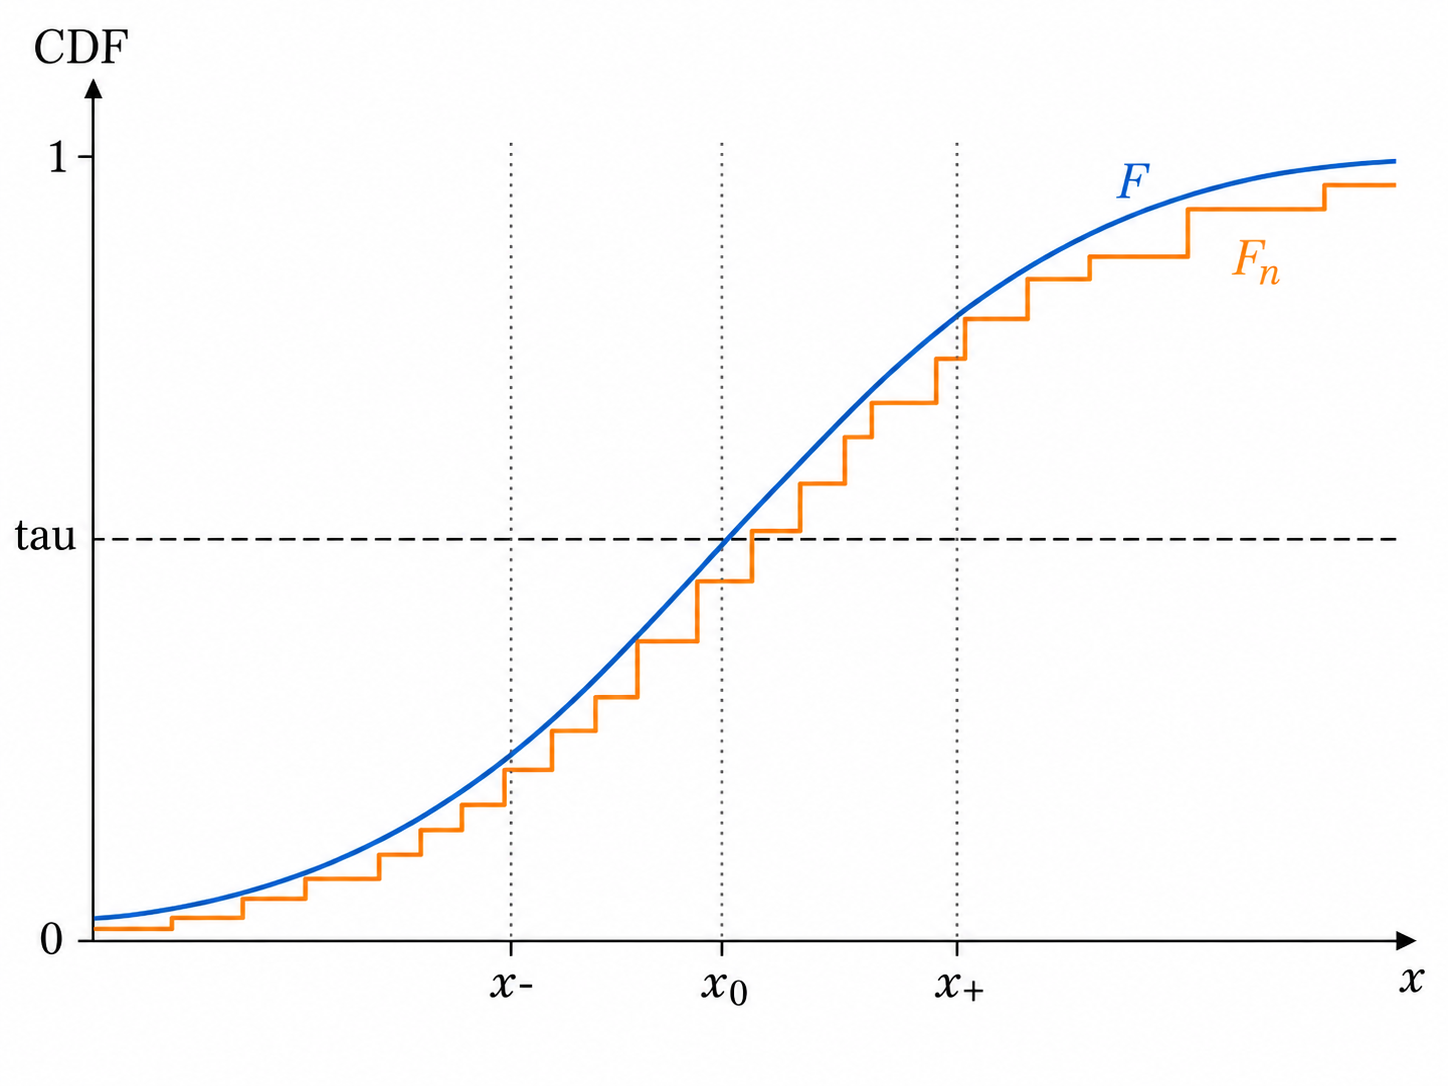
\includegraphics[width=0.78\textwidth]{./lec3-quantile-consistency-illustration.png}

  \small Uniform closeness of the two CDFs keeps the empirical $\tau$-quantile inside $[q-\varepsilon,q+\varepsilon]$.
\end{center}

Consequently,
\begin{align*}
  \Prob\bigl(|T_\tau(\widehat{F}_n)-q| > \varepsilon\bigr)
  \leq \Prob\Bigl(\sup_x |\widehat{F}_n(x)-F(x)| \geq \delta\Bigr) \longrightarrow 0,
\end{align*}
which proves consistency of the sample quantile.

Remark: when $\tau$ can change with $n$, we need to be more careful. For example, we can consider $\tau > 1 - 1/n$. In such a case, the sample quantile is
\begin{align*}
  T_\tau (\widehat{F}_n) = \max_{i=1, 2, \ldots, n} X_i.
\end{align*}
e.g. if we take $\tau = 1 - 1/n^2$, then population quantile at $1 - 1/n^2$ could be much larger than the sample maximum, and we do not have convergence. In general, we need to assume that $\tau$ is fixed and does not change with $n$.

\paragraph{Additional nonlinear functionals:}
Lipschitz functionals: we call a functional $T$ as $L$-Lipschitz if
\begin{align*}
  |T(F_1) - T(F_2)| \leq L \cdot \sup_{x \in \real} |F_1(x) - F_2(x)|,
\end{align*}
for some constant $L > 0$.

For Lipschitz functionals, we have
\begin{align*}
  |T(\widehat{F}_n) - T(F)| \leq L \cdot \sup_{x \in \real} |\widehat{F}_n(x) - F(x)| \xrightarrow{p} 0,
\end{align*}
We can also get quantitative bounds on the estimation error using DKW inequality.

This also applies to functionals that are H\"{o}lder continuous, or has some other modulus of continuity. In general, we can show that if $T$ is continuous with respect to the uniform norm, then the plug-in estimator works.

\begin{example}\upshape
  Consider the functional
  \begin{align*}
    T (F) \mydefn \max_{x \in \real} \Prob (X \in [x - 1, x + 1]) = \max_{x \in \real} (F(x + 1) - F(x - 1)).
  \end{align*}
  For two functions $F_1$ and $F_2$, we have
  $|\max_x a_x - \max_x b_x| \leq \sup_x |a_x-b_x|$. Hence
  \begin{align*}
    |T (F_1) - T (F_2)|
    &\leq \sup_{x \in \real} |(F_1-F_2)(x+1) - (F_1-F_2)(x-1)| \\
    &\leq 2 \sup_{x \in \real} |F_1(x) - F_2(x)|.
  \end{align*}
  So $T$ is a $2$-Lipschitz functional, and the plug-in estimator works.
\end{example}
If we study $\arg\max$ instead of $\max$, we need some additional assumption to guarantee that the argmax is unique, and then we can apply the same idea as what we did for quantile estimation to show convergence of the plug-in estimator.


\section{Bootstrap}
Idea: by uniform convergence of the CDF, we know that somehow $\widehat{F}_n \approx F$. In confidence interval construction, we need to quantify the uncertainty of the estimator $\widehat{T}_n = T(\widehat{F}_n)$, e.g.,
\begin{align*}
  \mathrm{se}_F (\widehat{T}_n) = \sqrt{\Exs_F \big[ | \widehat{T}_n - \Exs_F [\widehat{T}_n] |^2 \big]}.
\end{align*}
The problem is that this formula depends on unknown $F$. On the other hand, we can replace $F$ by $\widehat{F}_n$, and the estimated version of standard error is
\begin{align*}
   \mathrm{se}_{\widehat{F}_n} (\widehat{T}_n) = \sqrt{\Exs_{\widehat{F}_n} \big[ | \widehat{T}_n - \Exs_{\widehat{F}_n} [\widehat{T}_n] |^2 \big]}.
\end{align*}
Here, by subscript $\widehat{F}_n$, we mean that the expectation is taken with respect to the empirical distribution $\widehat{F}_n$. Empirical distribution is known to us, so we can compute this quantity in principle. This is the basic idea of bootstrap.

General idea:
\begin{itemize}
  \item Write the quantity of interest as a functional of the CDF $F$ (and the estimator).
  \item Replace $F$ by the empirical CDF $\widehat{F}_n$ to get an estimated version of the quantity of interest.
\end{itemize}

In other words, we can think of it as two ``parallel worlds'':
\begin{itemize}
  \item True distribution is $F$, and you get samples $X_1, X_2, \ldots, X_n \simiid F$. You can compute the estimator $\widehat{T}_n$ based on these samples.
  \item Hypothetical ``bootstrap world'': you pretend that the empirical distribution $\widehat{F}_n$ is the true distribution, and you generate bootstrap samples $X_1^*, X_2^*, \ldots, X_n^* \simiid \widehat{F}_n$. You can compute the bootstrap estimator $\widehat{T}_n^*$ based on these bootstrap samples.
\end{itemize}
Operationally, the bootstrap samples $X_1^*, X_2^*, \ldots, X_n^*$ can be generated by sampling with replacement from the original samples $X_1, X_2, \ldots, X_n$. We re-sampled the original samples.

\end{document}
